\documentclass[10pt,landscape]{article}
\usepackage[utf8]{inputenc}
\usepackage{multicol}
\usepackage{calc}
\usepackage{ifthen}
\usepackage[landscape]{geometry}
\usepackage{hyperref}
\usepackage{amsmath, amssymb, amsthm, bm, hyperref, float, mathtools}
% \usepackage{minted}
\usepackage{graphicx}
\usepackage{enumitem}
\usepackage{sectsty}

% Use images folder as root path for images
\graphicspath{ {images/} }

% Remove extra spacing on bullet points
\setlist[itemize]{nosep,leftmargin=*}

% This sets page margins to .5 inch if using letter paper, and to 1cm
% if using A4 paper. (This probably isn't strictly necessary.)
% If using another size paper, use default 1cm margins.
\ifthenelse{\lengthtest { \paperwidth = 11in}}
    { \geometry{top=.5in,left=.5in,right=.5in,bottom=.5in} }
    {\ifthenelse{ \lengthtest{ \paperwidth = 297mm}}
        {\geometry{top=1cm,left=1cm,right=1cm,bottom=1cm} }
        {\geometry{top=1cm,left=1cm,right=1cm,bottom=1cm} }
    }

% Turn off header and footer
\pagestyle{empty}


% Redefine section commands to use less space
\makeatletter

\sectionfont{\normalsize}
\subsectionfont{\small}
\subsubsectionfont{\small}
\paragraphfont{\small}

% \renewcommand{\section}{\@startsection{section}{1}{0mm}%
%                                 {-1ex plus -.5ex minus -.2ex}%
%                                 {0.5ex plus .2ex}%x
%                                 {\normalfont\normalsize\bfseries}}
% \renewcommand{\subsection}{\@startsection{subsection}{2}{0mm}%
%                                 {-1ex plus -.5ex minus -.2ex}%
%                                 {0.5ex plus .2ex}%
%                                 {\normalfont\small\bfseries}}
% \renewcommand{\subsubsection}{\@startsection{subsubsection}{3}{0mm}%
%                                 {-1ex plus -.5ex minus -.2ex}%
%                                 {1ex plus .2ex}%
%                                 {\normalfont\small\bfseries}}
\makeatother

% Define BibTeX command
\def\BibTeX{{\rm B\kern-.05em{\sc i\kern-.025em b}\kern-.08em
    T\kern-.1667em\lower.7ex\hbox{E}\kern-.125emX}}

% Don't print section numbers
\setcounter{secnumdepth}{0}

\setlength{\parindent}{0pt}
\setlength{\parskip}{0pt plus 0.5ex}

% -----------------------------------------------------------------------

\DeclarePairedDelimiter{\ceil}{\lceil}{\rceil}
\newcommand{\expect}[1]{\mathbf{E}[#1]}
\newcommand{\var}[1]{\text{Var(#1)}}
\newcommand{\cov}[1]{\text{Cov(#1)}}
\newcommand{\identity}{\mathbf{I}}

% -----------------------------------------------------------------------

\begin{document}

\raggedright
\footnotesize
\begin{multicols}{3}

\setlength{\premulticols}{1pt}
\setlength{\postmulticols}{1pt}
\setlength{\multicolsep}{1pt}
\setlength{\columnsep}{2pt}

% =============================================================================

\section{Sampling}

\textit{Antialiasing}: Removing frequencies above the Nyquist frequency (2 times the highest frequency) before sampling. Done by filtering before sampling. \\
\textit{Line equation}: $L(x, y) = Ax + By + C$. On line: $L(x, y) = 0$, on right: $L(x, y) > 0$, on left: $L(x, y) < 0$. A point is inside a convex polygon if line tests for all lines (going clockwise) is greater than 0.

\textit{Fourier transform}: $F(\omega) = \int_{-\infty}^{\infty} f(x) e^{-2\pi i \omega x} \,dx$ \\
\textit{Inverse transform}: $f(x) = \int_{-\infty}^{\infty} F(\omega) e^{2\pi i \omega x} \,d\omega$ \\
\textit{Euler's formula}: $e^{ix} = \cos x + i\sin x$

% =============================================================================

\section{Transforms}

\textit{Homogeneous coordinates}: Points are defined as $(x, y, 1)$ and vectors by $(x, y, 0)$. Points and vectors don't reside on the same $xy$ plane. \\
\textit{Affine transformations}: Consist of linear map and a translation. \\
\textit{Camera transformations}: Given eye point $e$, up vector $u$, view direction $v$, where $u$ and $v$ are orthonormal, find right vector $r = v \times u$. Transform camera $(e, r, u, v)$ to standard camera located at the origin, looking down the negative $z$-axis, where the up vector is the $y$-axis.

\subsection{Transform Order}

\begin{itemize}[nosep]
    \item Object coordinates: Apply modeling transforms
    \item World (scene) coordinates: Apply viewing transform
    \item Camera (eye) coordinates: Apply perspective transform and homogeneous division
    \item Normalized device coordinates: Apply 2D screen transform
    \item Screen coordinates: Rasterization
\end{itemize}

\subsection{Basic Transformations}

\begin{multicols}{2}

Scaling

$$\begin{bmatrix}
s & 0 & 0 \\
0 & s & 0 \\
0 & 0 & 1
\end{bmatrix}$$

Rotation

$$\begin{bmatrix}
\cos(\theta) & -\sin(\theta) & 0 \\
\sin(\theta) & \cos(\theta) & 0 \\
0 & 0 & 1
\end{bmatrix}$$

\columnbreak

Translation

$$\begin{bmatrix}
1 & 0 & t_x \\
0 & 1 & t_y \\
0 & 0 & 1
\end{bmatrix}$$

Shear

$$\begin{bmatrix}
1 & \lambda & 0 \\
0 & 1 & 0 \\
0 & 0 & 1
\end{bmatrix}$$

\end{multicols}

\subsection{Coordinate System Transform}

Frame-to-world transformation converts frame axes to world axes centered at origin with $x$ mapped to $u$ and $y$ mapped to $v$.

\begin{align*}
    F &= \begin{bmatrix}
        \textbf{u} & \textbf{v} & \textbf{o}
    \end{bmatrix} \\
    &= \begin{bmatrix}
        u_x & v_x & o_x \\
        u_y & v_y & o_y \\
        0 & 0 & 1
    \end{bmatrix}
\end{align*}

Rotation by angle $\alpha$ around axis $n$:

$$\cos(\alpha)\identity + (1 - \cos(\alpha))nn^T + \sin(\alpha)\begin{bmatrix}
    0 & n_z & -n_y \\
    -n_z & 0 & n_x \\
    n_y & -n_x & 0
\end{bmatrix}$$

\subsection{Hierarchical Transform}

\subsection{Projective Transform}

Project some point in the scene $(x, y, z)^T$ to a point on the image plane. If the center of projection is at $(0, 0, 0)^T$ and the image plane is at $z = d$, then $(x, y, z)^T \rightarrow (xd/z, yd/z, d)^T$.

Requires division by $z$, so use homogeneous coordinates:

$$
q = \begin{bmatrix}
        1 & 0 & 0 & 0 \\
        0 & 1 & 0 & 0 \\
        0 & 0 & 1 & 0 \\
        0 & 0 & 1/d & 0
    \end{bmatrix}
    \begin{bmatrix}
        x \\
        y \\
        z \\
        1
    \end{bmatrix} =
    \begin{bmatrix}
        xd/z \\
        yd/z \\
        d \\
        1
    \end{bmatrix}
$$

\subsection{Perspective Projection}

Parameterized by: \textit{fovy}: vertical angular field of view, \textit{aspect}: width/height of field of view, \textit{near}: depth of near clipping plane, \textit{far}: depth of far clipping plane

Derived quantities: $top = near \cdot \tan(fovy)$, $bottom = -top$, $right = top \cdot aspect$, $left = -right$

Convert from camera coordinates to normalized device coordinates (NDC) by mapping the view volume frustum into a cube, where $(left, bottom, -near) \rightarrow (-1, -1, -1)$ and $(right, top, -far) \rightarrow (1, 1, 1)$. Linear transformation in homogeneous coordinates.

$$\begin{bmatrix}
    \frac{near}{right} & 0 & 0 & 0 \\
    0 & \frac{near}{top} & 0 & 0 \\
    0 & 0 & -\frac{far+near}{far-near} & \frac{-2(far\cdot near)}{far-near}\\
    0 & 0 & -1 & 0
\end{bmatrix}$$

% =============================================================================

\section{Texture Mapping}

\subsection{Barycentric Coordinates}

Linearly interpolate values at vertices for a point in the triangle

$$(x, y) = \alpha A + \beta B + \gamma C$$
$$\alpha + \beta + \gamma = 1$$

\begin{multicols}{3}

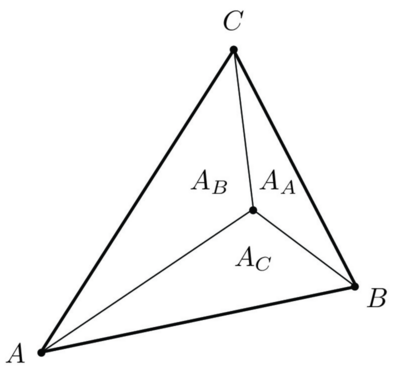
\includegraphics[scale=0.2]{barycentric_area}

\columnbreak

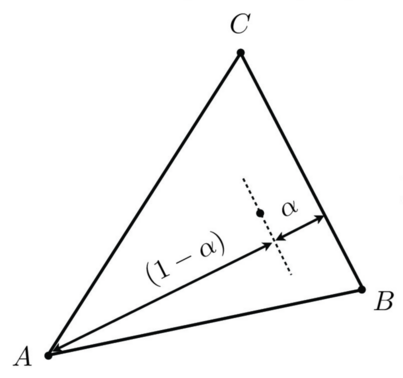
\includegraphics[scale=0.18]{barycentric_ratio}

\end{multicols}

\begin{align*}
    \alpha &= \frac{-(x - x_B)(y_C - y_B) + (y - y_B)(x_C - x_B)}{-(x_A - x_B)(y_C - y_B) + (y_A - y_B)(x_C - x_B)} \\
    \beta &= \frac{-(x - x_C)(y_A - y_C) + (y - y_C)(x_A - x_C)}{-(x_B - x_C)(y_A - y_C) + (y_B - y-C)(x_A - x_C)} \\
    \gamma &= 1 - \alpha - \beta
\end{align*}

\begin{multicols}{3}
    $\alpha &= \frac{A_A}{A_A + A_B + A_C}$
    \columnbreak
    $\beta &= \frac{A_B}{A_A + A_B + A_C}$
    \columnbreak
    $\gamma &= \frac{A_C}{A_A + A_B + A_C}$
\end{multicols}

\subsection{Texture Sampling}

Affine screen-space interpolation doesn't work, because linear interpolation in world coordinates yields nonlinear interpolation in screen coordinates.

\textit{Magnification}: Each pixel is a small part of the texel. \\ \textit{Minification}: each pixel includes many texels, leading to aliasing.

\subsection{Mipmaps}

Filter before sampling; use resolution that matches screen sampling rate. Estimate texture footprint using texture coordinates of neighboring screen samples, then use that to figure out which level of mipmap to use.

$$D = \log_2 L$$

$$L = max\left(\sqrt{\left(\frac{du}{dx}\right)^2 + \left(\frac{dv}{dx}\right)^2}, \sqrt{\left(\frac{du}{dy}\right)^2 + \left(\frac{dv}{dy}\right)^2}\right)$$

\textit{Anisotropic filtering}: Mipmaps change depending on viewing angle. One way is to generate more mipmaps with variations on both $x$ and $y$, instead of just taking the max of both.

% =============================================================================

\section{Graphics Pipeline}

\textit{Lambert's cosine law}: Light per unit area is proportional to $\cos(\theta) = I \cdot n$, where $\theta$ is the angle between the normal and the light source and $I$ is a vector from hit point to light source. \\
\textit{Lambertian (Diffuse) shading}: Shading independent of view direction. $L_d = k_d (I / r^2) max(0, n\cdot l)$ \\
\textit{Specular shading}: Close to mirror at the half-vector near normal. $h = \text{bisector}(v, l) = \frac{v + l}{\Vert v + l \Vert}$ \\
$L_s = k_s(I / r^2) \max(0, n \cdot h)^p$ \\
\textit{Ambient shading}: doesn't depend on anything, adds constant color to account for disregarded illumination and fill in black shadows. Not physically accurate, since it's not based on any incoming radiance. $L_a = k_a I_a$

% =============================================================================

\section{Intro to Geometry}

\textit{Implicit geometry}: Surface defined where $f(x, y, z) = 0$. Can test if point is inside or outside easily, but hard to sample (what points lie on the surface?) Description can be compact, good for ray-to-surface intersections. No sampling error, easy to handle changes in topology. Hard to model complex shapes. \\
\textit{Explicit geometry}: All points given directly, $f : \mathbb{R}^2 \rightarrow \mathbb{R}^3; (u, v) \rightarrow (x, y, z)$. Sampling easy, but hard to tell if point is inside/outside surface. \\
\textit{Topological validity}: A 2D manifold is a surface that when cut with a sphere always yields a disk. Mesh manifolds always have the properties: edge connects two faces and two vertices, face consists of ring of edges and vertices, vertex consists of ring of edges and faces. $F - E + V = 2$ holds for a surface topologically equivalent to a sphere.

\begin{multicols}{2}
\begin{verbatim}
struct Halfedge {
    Halfedge *twin;
    Halfedge *next;
    Vertex *vertex;
    Edge *edge;
    Face *face; }
\end{verbatim}

\columnbreak

\begin{verbatim}
struct Vertex {
    Halfedge *halfedge; }
struct Edge {
    Halfedge *halfedge; }
struct Face {
    Halfedge *halfedge; }
\end{verbatim}
\end{multicols}

\textit{Loop subdivision}: Split edges of original mesh in any order, then flip new edges that touch a new and old vertex.

% =============================================================================

\section{Splines, Curves, and Surfaces}

\subsection{Cubic Polynomial Interpolation}

\begin{align*}
    P(t) &= at^3 + bt^2 + ct + d \\
    P^{\prime}(t) &= 3at^2 + 2bt + c
\end{align*}

Hermite matrix:

\begin{align*}
    P(t) &= at^3 + bt^2 + ct + d \\
    &=  \begin{bmatrix}
            t^3 & t^2 & t & 1
        \end{bmatrix}
        \begin{bmatrix}
            2 & -2 & 1 & 1 \\
            -3 & 3 & -2 & -1 \\
            0 & 0 & 1 & 0 \\
            1 & 0 & 0 & 0
        \end{bmatrix}
        \begin{bmatrix}
            h_0 \\
            h_1 \\
            h_2 \\
            h_3
        \end{bmatrix} \\
    &= H_0(t)h_0 + H_1(t)h_1 + H_2(t)h_2 + H_3(t)h_3
\end{align*}

\begin{align*}
    H_0(t) &= 2t^3 - 3t^2 + 1 \\
    H_1(t) &= -2t^3 + 3t^2 \\
    H_2(t) &= t^3 - 2t^2 + t \\
    H_3(t) &= t^3 - t^2
\end{align*}

\subsection{Bezier Curves}

$$B_i^n(t) = \binom{n}{i} t^i (1-t)^{n-i}$$

\begin{align*}
    P(t) &= \sum_{i=0}^3 P_i B_i(t) \\
    &= (1-t)^3 P_0 + 3t(1-t)^2 P_1 + 3t^2(1-t) P_2 + t^3 P_3 \\
    &=  \begin{bmatrix}
            (1-t)^3 & 3t(1-t) & 3t^2(1-t) & t^3
        \end{bmatrix}
        \begin{bmatrix}
            P_0 \\
            P_1 \\
            P_2 \\
            P_3
        \end{bmatrix} \\
    &=  \begin{bmatrix}
            1 & t & t^2 & t^3
        \end{bmatrix}
        \begin{bmatrix}
            1 & 0 & 0 & 0 \\
            -3 & 3 & 0 & 0 \\
            3 & -6 & 3 & 0 \\
            -1 & 3 & -3 & 1
        \end{bmatrix}
        \begin{bmatrix}
            P_0 \\
            P_1 \\
            P_2 \\
            P_3
        \end{bmatrix}
\end{align*}

\subsubsection{de Casteljau Algorithm}

% 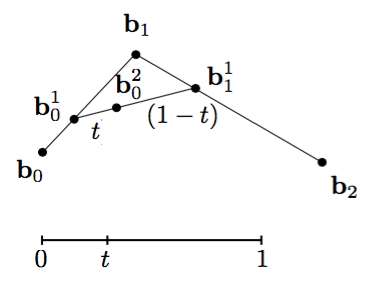
\includegraphics[scale=0.2]{decasteljau}

\begin{align*}
    B(t) &= (1-t)((1-t)P_0 + tP_1) + t((1-t)P_1 + tP_2) \\
    &= (1-t)^2 P_0 + 2t(1-t)P_1 + t^2 P_3 \\
    &=  \begin{bmatrix}
            (1-t)^2 & 2t(1-t) & t^2
        \end{bmatrix}
        \begin{bmatrix}
            P_0 \\
            P_1 \\
            P_2
        \end{bmatrix} \\
    &=  \begin{bmatrix}
            1 & t & t^2
        \end{bmatrix}
        \begin{bmatrix}
            1 & 0 & 0 \\
            -2 & 2 & 0 \\
            1 & -2 & 1
        \end{bmatrix}
        \begin{bmatrix}
            P_0 \\
            P_1 \\
            P_2
        \end{bmatrix}
\end{align*}

$$b_{i,j}^{r,r} =
\begin{bmatrix}
    1 - u & u
\end{bmatrix}
\begin{bmatrix}
    b_{i, j}^{r-1, r-1} & b_{i, j+1}^{r-1, r-1} \\
    b_{i+1, j}^{r-1, r-1} & b_{i+1, j+1}^{r-1, r-1}
\end{bmatrix}
\begin{bmatrix}
    1 - v \\
    v
\end{bmatrix}$$

% =============================================================================

\section{Geometry Processing}

\subsection{Catmull-Clark Vertex Update}

$$f = \frac{v_1 + v_2 + v_3 + v_4}{4} \qquad e = \frac{v_1 + v_2 + f_1 + f_2}{4}$$

% =============================================================================

\section{Accelerating Ray Tracing}

Ray: $r(t) = o + td, 0 \le t < \infty$ \\
General implicit surface: $p: f(p) = 0$ \\
Substitute ray equation: $f(o + td) = 0$ \\
Sphere: $(p - c)^2 - R^2 = 0$

$$t = \frac{(p - o) \cdot N}{d \cdot N} \rightarrow \frac{p_x - o_x}{d_x}$$

% =============================================================================

\section{Radiometry and Photometry}

\textit{Radiant Flux} \\
\textit{Radiant Intensity}: Power per unit solid angle emitted from a point light source. \\
\textit{Irradiance}: Power per unit area $(W/m^2)$., follows Lambert's cosine law, irradiance falloff follows inverse square law \\
\textit{Radiance}: Power per unit area per unit solid angle $(W/sr/m^2)$.

% =============================================================================

\section{Monte Carlo Integration}

$$F_N = \frac{1}{N} \sum_{i=1}^N \frac{f(x_i)}{p(x_i)}$$

\subsection{Inversion method}

Given $P(x) = Pr(X < x)$, solve for $x = P^{-1}(\xi)$. Need to know the integral of the PDF $p(x)$ for this to work. Example:

$$p_\lambda(x) = \lambda e^{-\lambda x}$$

$$\begin{aligned}
F(t) = P_\lambda(X \le t) &= \int_0^t \lambda e^{-\lambda x} dx \\
                          &= 1 - e^{-\lambda t}
\end{aligned}$$

$$F^{-1}(\xi) = \frac{-\log(1 - \xi)}{\lambda}$$

\subsection{Expectation and Variance}

\begin{align*}
    \expect{X + c} &= \expect{X} + c \\
    \expect{X + Y} &= \expect{X} + \expect{Y} \\
    \expect{aX} &= a\expect{X}
\end{align*}

\begin{align*}
    \var{X + a} &= \var{X} \\
    \var{aX} &= a^2 \var{X} \\
    \var{aX + bY} &= a^2 \var{X} + b^2 \var{Y} + 2ab \cov{X, Y}
\end{align*}

% =============================================================================

\section{Reflection and Materials}

\textit{Bidirectional Reflectance Distribution (BRDF)}: Non-negative (always returns a positive value for any input ray), respects linearity, reciprocity principle: $f_r(w_i \rightarrow w_r) = f_r(w_r \rightarrow w_i)$, conserves energy.

% =============================================================================

\end{multicols}
\end{document}
